\section{Symbolic Computing}
\subsection{Limitations of Existing}
\gls{symengine} and \gls{sympy} are great for mathematics but not for generating high performance code.

\subsubsection{Multiple Outputs}
Vector instructions.
SinCos.

\subsubsection{Context Awareness}
a/x -> a/x,   a/x, b/x -> r = 1/x, a*r, b*r

\subsection{Hardware Oriented Code Generation}
Use available acceleratost, e.g. norm functions.


\subsection{Adaptive Reordering}
Each thread on the GPU has a finite set of 32-bit registers available.
If a kernel need more registers than whats available, local memory is used.
Ther is called register spilling an has a negative on performance, as local memory is as slow as global memory.
To minimize the amount of register spilling we want to find an optimal expression ordering.
This problem is called the bandwidth minimization problem and is NP-hard.
\begin{figure}[H]
    \centering
    \begin{tabular}[b]{ccc}

        \subcaptionbox{Array of scalars}{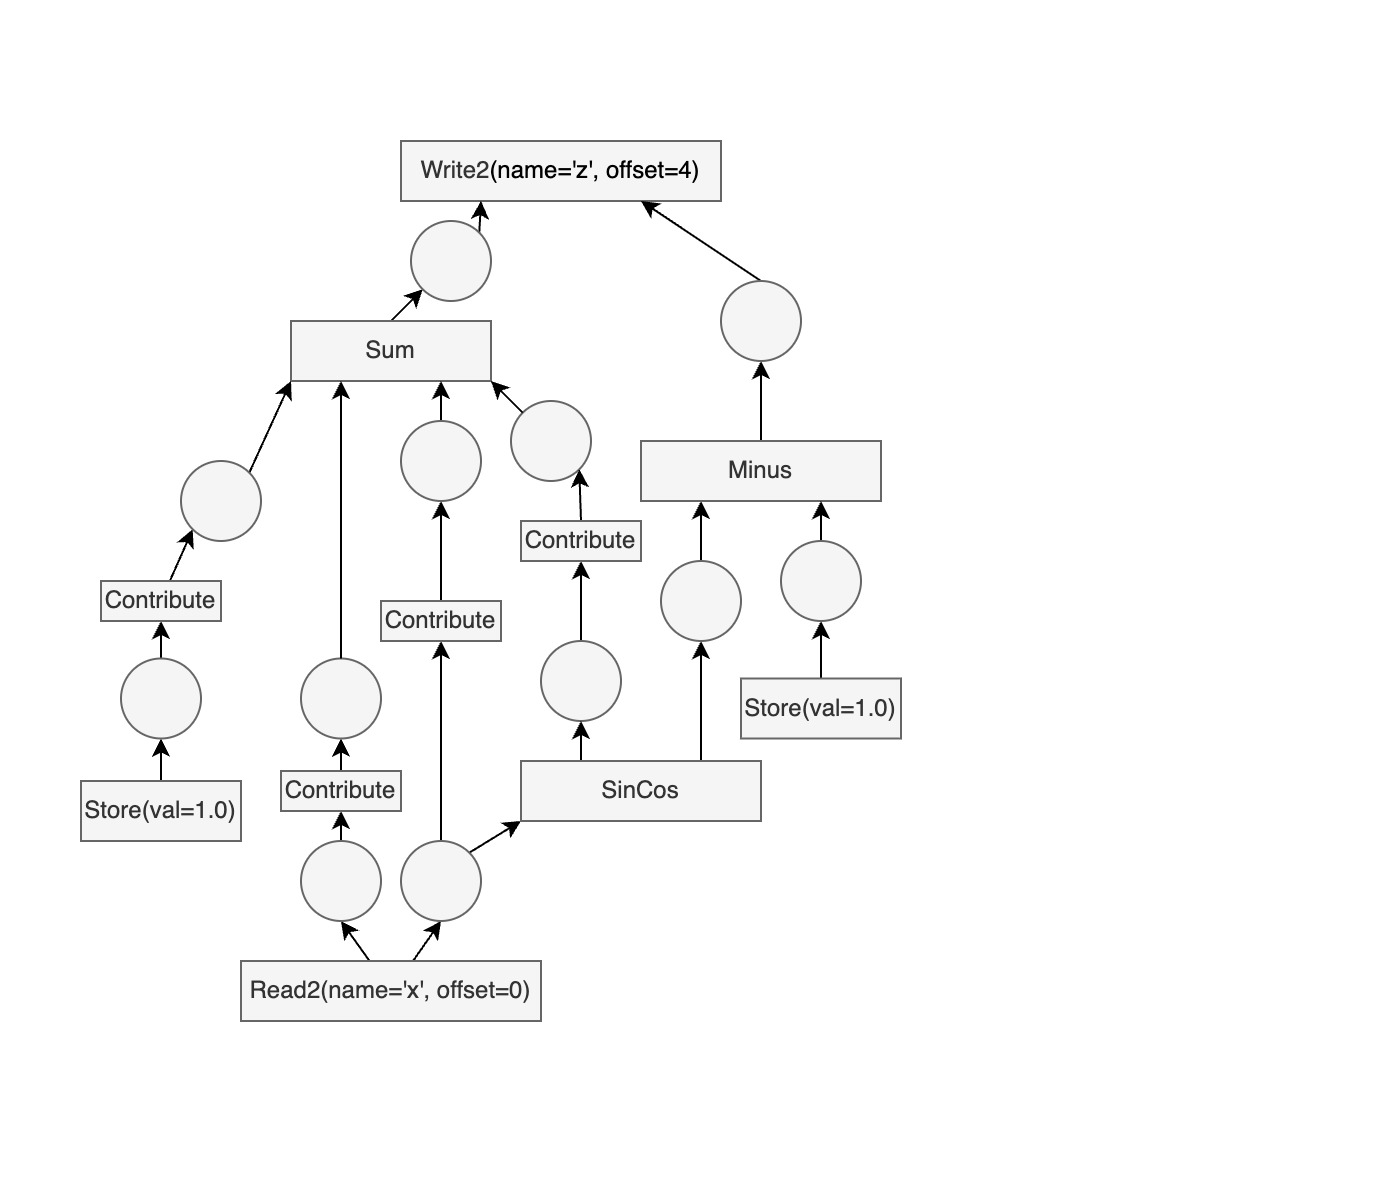
\includegraphics[trim={2.5cm 5cm 16cm 4cm},clip,width=0.5\textwidth]{figures/code_generation_example/symbolic_ordering-0.png}
        }
         &
        \subcaptionbox{Array of scalars}{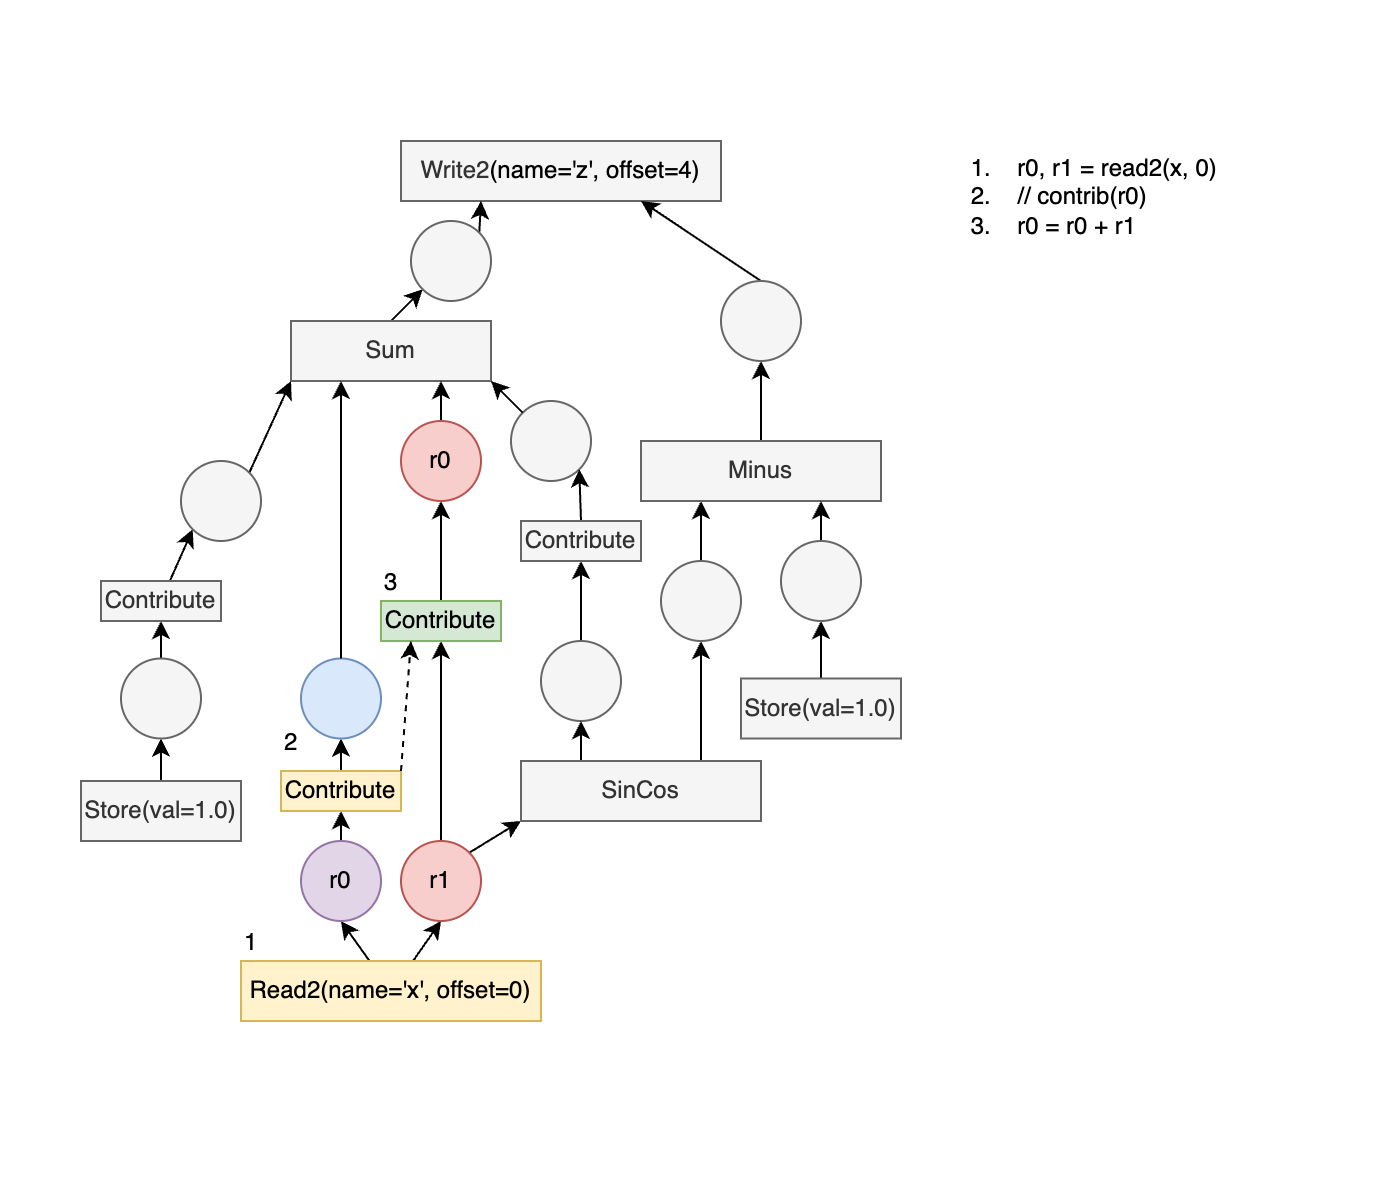
\includegraphics[trim={2.5cm 5cm 16cm 4cm},clip,width=0.5\textwidth]{figures/code_generation_example/symbolic_ordering-3.png}
        }
        \\ \vspace{0.5cm} \\
        \subcaptionbox{Array of scalars}{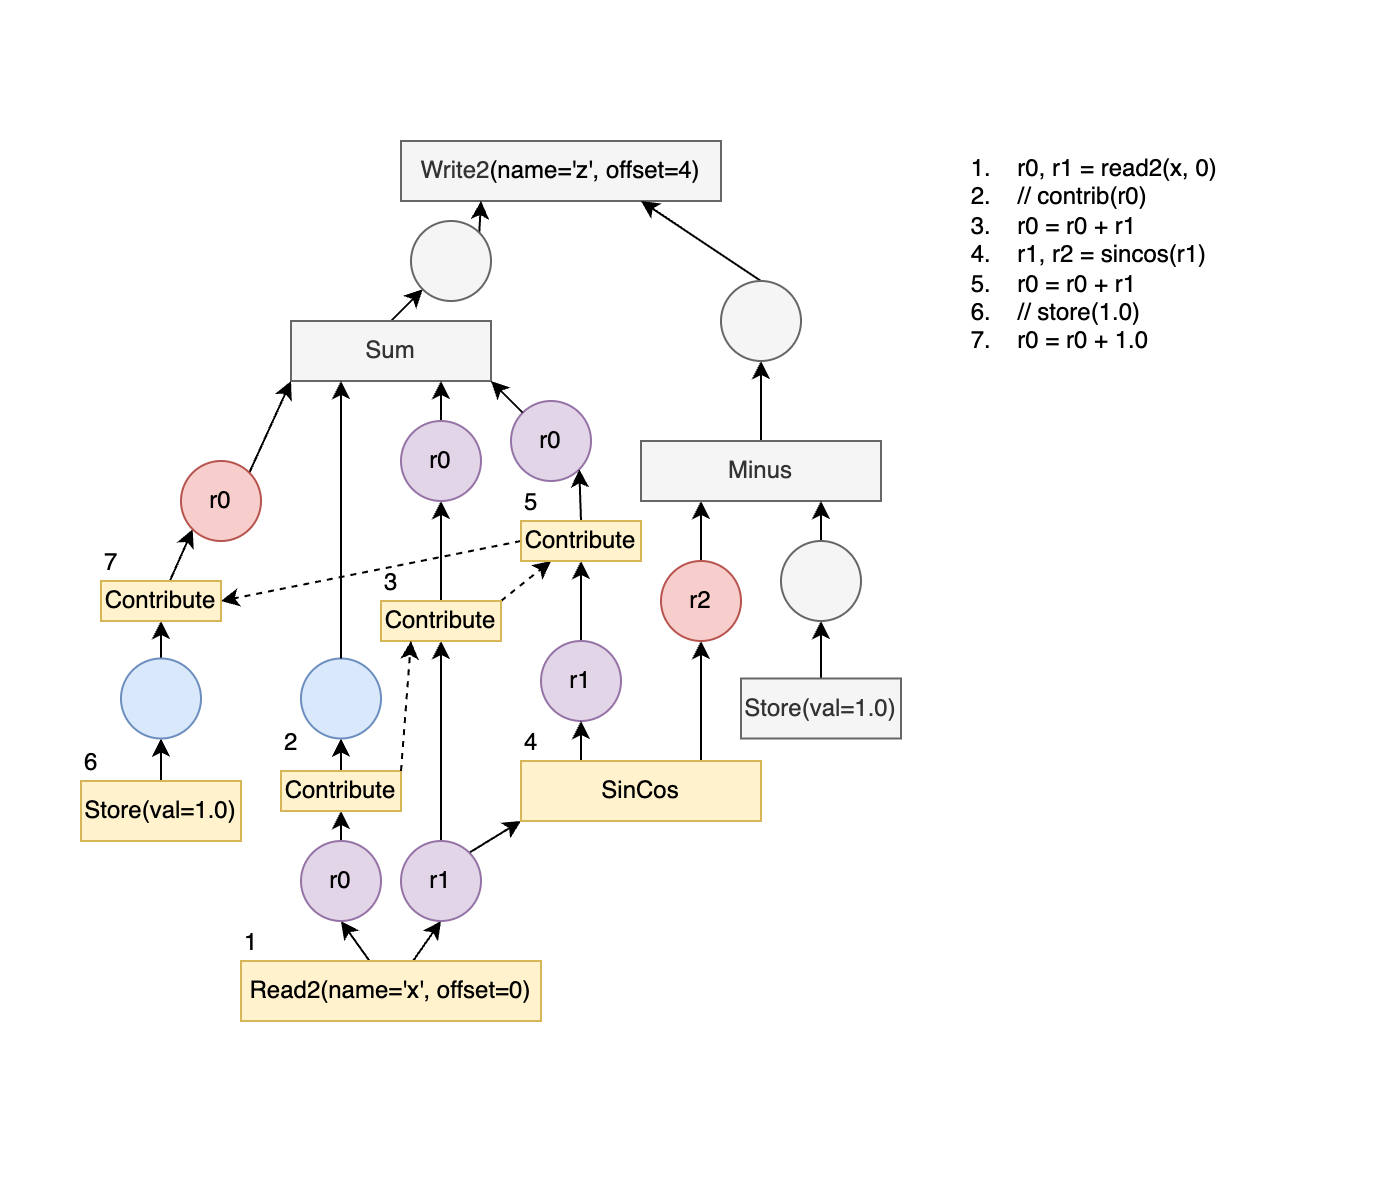
\includegraphics[trim={2.5cm 5cm 16cm 4cm},clip,width=0.5\textwidth]{figures/code_generation_example/symbolic_ordering-7.png}
        }

         &
        \subcaptionbox{Array of scalars}{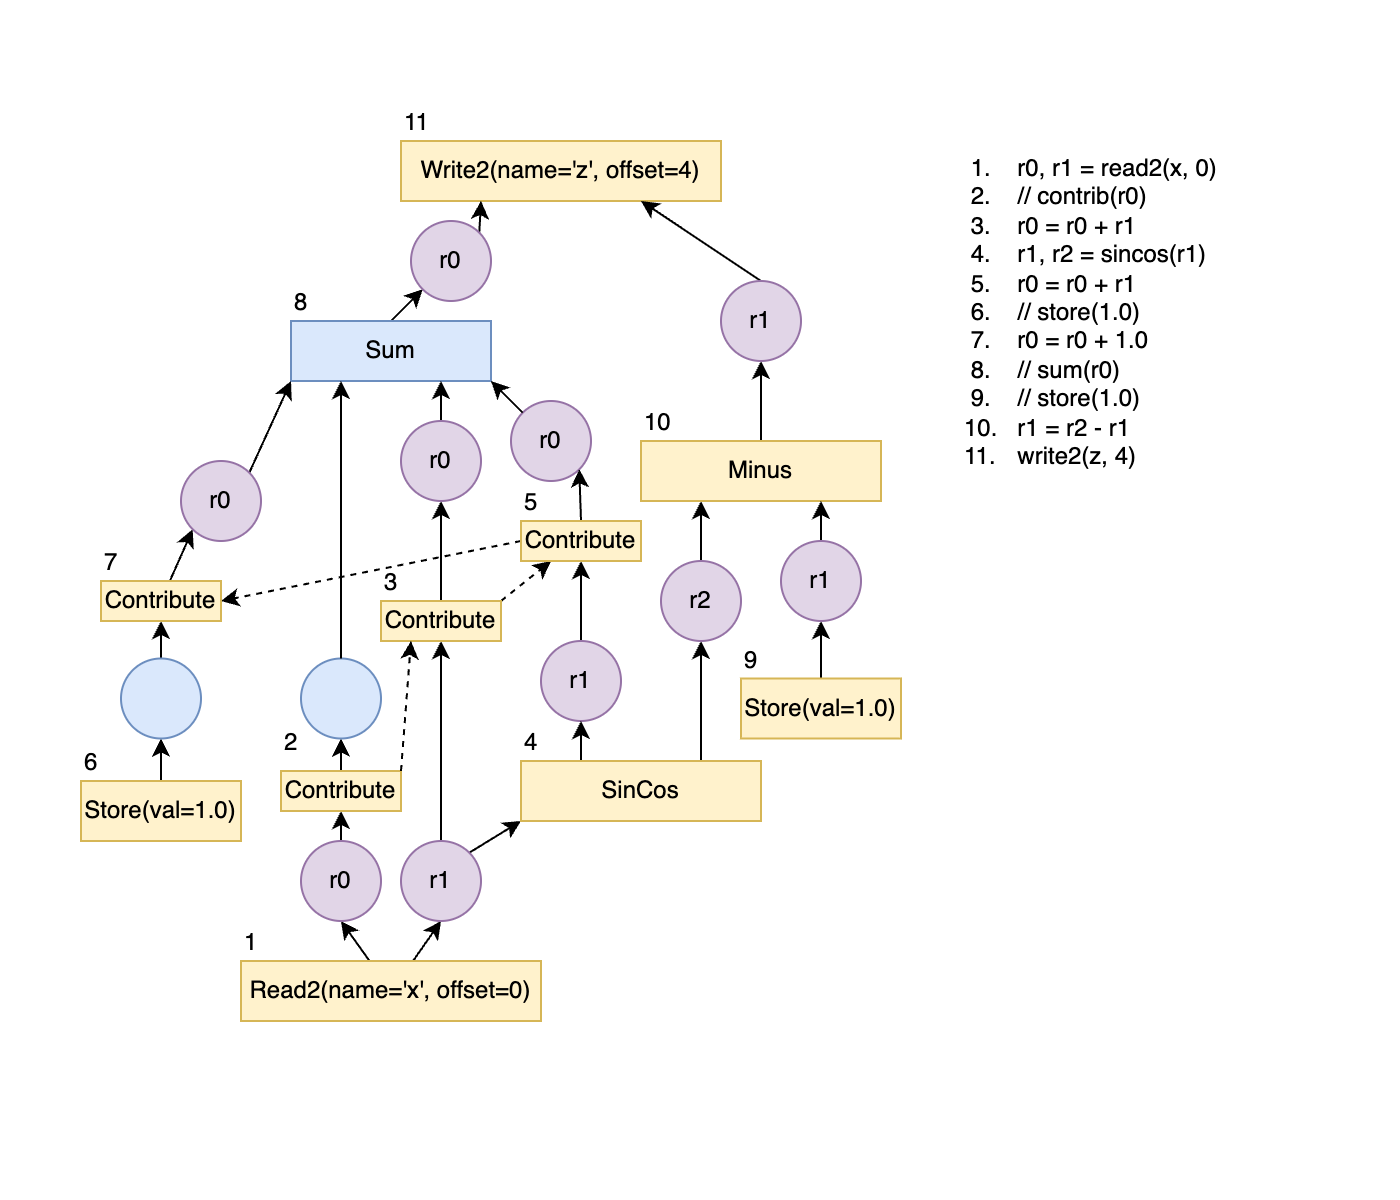
\includegraphics[trim={2.5cm 5cm 16cm 4cm},clip,width=0.5\textwidth]{figures/code_generation_example/symbolic_ordering-11.png}
        }

        \\
    \end{tabular}
    \caption{Mapping of arrays of structs with different number of fields. Fields are grouped into chunks of four as far as possibe, the remaning fields are appended at the end as chunks of the remaning size. All chunks are aligned to the number of bytes needed for the corresponding vector instruction.}
\end{figure}

